\documentclass[11pt]{article}

\usepackage[letterpaper,top=2cm,bottom=2cm,left=2.5cm,right=2.5cm,marginparwidth=1.75cm]{geometry}

%packages
\usepackage{amsmath}
\usepackage{graphicx}
\usepackage{amssymb}
\usepackage{algorithm}
\usepackage{algpseudocode}
\usepackage{color,soul}
\usepackage{mathtools}
% \usepackage{subfig}
\usepackage{subcaption}
\usepackage{caption}


% Edits by John:
% Use hyperref when you're referencing anything - in particular, use the \autoref{} command - it's great. One exception: anything in mathmode should be referenced using \eqref{} instead; \autoref{} calls all mathmode objects "equations", even when they're not equations (definitions, inequalities, propositions, statements, etc.), so it's better to use the \eqref{} function.
\usepackage[colorlinks, linkcolor=blue, citecolor=blue, urlcolor=blue]{hyperref}
% Use the align (or similar) environment, rather than built-in latex commands for math statements. That way, things can be aligned properly and equations will be numbered and referencable. The equation below assigns equation numbers based upon the current section.

\numberwithin{equation}{section}
% Use the amsthm environents to define theorems, remarks, definitions, etc., with commands of the form \begin{definition}[DEFINITION ITTLE]
\usepackage{amsthm}% provides the environments
\theoremstyle{definition}% provides a style for definitions - this affects all downstream \newtheorem statements until \theoremstyle is used again.
\newtheorem{theorem}{Theorem}
\newtheorem{definition}{Definition}[section]% numbers definitions within sections
% The singular of "matrices" is "matrix", not "matrice" - the abnormal singular-plural pair is an importation from Latin.
% Use \url{} for hyperlinks (I changed the pytorch link). I think this is included in hyperref, but it may be in base LaTeX.

\DeclarePairedDelimiter\ceil{\lceil}{\rceil}
\DeclarePairedDelimiter\floor{\lfloor}{\rfloor}
\newcommand{\pluseq}{\mathrel{+}=}
\newcommand{\asteq}{\mathrel{*}=}
\newcommand{\Loss}{L}

\usepackage[dvipsnames]{xcolor}
\usepackage[many]{tcolorbox}

\definecolor{lavender}{RGB}{214, 111, 208}
\colorlet{lavender}{lavender!50}

\newcommand{\hlinfo}[1]{{\sethlcolor{lavender}\hl{#1}}}
\newcommand{\note}[1]{\textcolor{red}{[#1]}}

\usepackage{tikz}


\newcommand{\framedbox}[1]{
    \noindent{\centering\framebox{\parbox{\linewidth - 0.75em}{#1}}\par}\vspace{0.5ex}
}
\newcommand{\resource}[1]{
\framedbox{\textbf{Resource:} #1}
}

\def\arraystretch{1.5} % padding table

\setlength\parindent{0pt}
\font\smallheader=cmr12 at 4pt


\begin{document}

\noindent
\title{Lecture Notes\\\vspace{0em}
\large Lectures 3 \& 4\\
\normalsize \emph{CS389: Machine Learning, Spring 2023}\\
\emph{University of Massachusetts Amherst}
\date{\smallheader}
}
\maketitle

\section{Multilayer Perceptrons (lecture 5)}

\subsection{Non-linearities}

% It means that the neural network can successfully approximate functions that do not follow linearity or it can successfully predict the class of a function that is divided by a decision boundary which is not linear
% Hopefully, a neural network with a non-linear activation function will allow the model to create complex mappings between the network’s inputs and outputs. 

In a previous lecture, we mentioned that the perceptron is unable to solve a dataset that is not linearly separable (e.g XOR). Adding more layers to the network, without any non-linear functions, will be ineffecitve because the model with many layers is still linear and could still be represented as a single layer perceptron.

\begin{align}
    W_m(W_{m-1}(W_{m-2}(\cdots W_{1} X))) = WX
\end{align}

Another way we can show this is that if we have 2 distinct linear models $g(x)$ and $f(x)$, then $f(g(x))$ is a linear model that is equivalent to some other linear function $h(x)$, think composite functions.
\begin{align}
    h(x) = f(g(x))
\end{align}

To approximate functions that do not follow linearity, we will introduce the concept of non-linear functions. Non-linearity will allow us to create non-linear mappings between the inputs and outputs. The most commonly used non-linear functions are the \emph{sigmoid}, \emph{tanh}, and \emph{ReLU} functions. Other non-linear functions may have different properties and may be useful for specific tasks, but sigmoid, tanh, and ReLU have become popular choices because they are simple, continuous, differentiable, and have other desirable properties for neural networks.



\subsubsection{Sigmoid}

\begin{figure}[h]
    \begin{center}
        \begin{subfigure}{0.35\textwidth}
            \includegraphics[width=4cm]{./Figs/sigmoid.png}%
        \label{fig:sigmoid_graph}
        \end{subfigure}
        \begin{subfigure}{0.35\textwidth}
            \begin{tabular}{||c c||} 
                \hline
                Non-linearity Function & Derivative \\ [0.5ex] 
                \hline
                $\sigma(x) = \frac{1}{1+e^{-x}}$ & $\sigma(x) \cdot [1-\sigma(x)]$ \\ [1ex] 
                \hline
            \end{tabular}
        \label{fig:sigmoid_math}
        \end{subfigure}
    \end{center}
    \caption{Sigmoid Function}
    \label{fig:sigmoid}
\end{figure}

The sigmoid function takes a real-valued number and “squashes” it into range between 0 and 1. In particular, large negative numbers become 0 and large positive numbers become 1. The sigmoid function has seen frequent use historically since it has a nice interpretation as the firing rate of a neuron: from not firing at all (0) to fully-saturated firing at an assumed maximum frequency (1). In practice, the sigmoid non-linearity has recently fallen out of favor and it is rarely ever used. It has two major drawbacks:

\begin{itemize}
    \item {\emph{Vanishing Gradients}. A very undesirable property of the sigmoid neuron is that when the neuron's activation saturates at either tail of 0 or 1, the gradient at these regions is almost zero. Therefore, if the local gradient is very small, it will effectively “kill” the gradient and almost no signal will flow through the neuron to its weights and recursively to its data. Additionally, one must pay extra caution when initializing the weights of sigmoid neurons to prevent saturation. For example, if the initial weights are too large then most neurons would become saturated and the network will barely learn.}
    \item {\emph{Outputs not zero-centered}.  This has implications on the dynamics during gradient descent, because if the data coming into a neuron is always positive, then the gradient on the weights $w$ will during backpropagation become either all be positive, or all negative.}
\end{itemize}


\subsubsection{Tanh}
The tanh function squashes a real-valued number to the range [-1, 1]. Like the sigmoid neuron, its activations saturate, but unlike the sigmoid neuron its output is zero-centered. Therefore, in practice the tanh non-linearity is always preferred to the sigmoid nonlinearity.

\begin{figure}[h]
    \begin{center}
        \begin{subfigure}{0.35\textwidth}
            \includegraphics[width=4cm]{./Figs/tanh.png}%
        \label{fig:tanh_graph}
        \end{subfigure}
        \begin{subfigure}{0.35\textwidth}
            \begin{tabular}{||c c||} 
                \hline
                Non-linearity Function & Derivative \\ [0.5ex] 
                \hline
                $\text{tanh}(x) = \frac{\text{sinh}(x)}{\text{cosh}(x)} = \frac{e^{x}-e^{-x}}{e^{x}+e^{-x}}$ & $1 - \text{tanh}^{2}(x)$ \\ [1ex] 
                \hline
            \end{tabular}
        \label{fig:tanh_math}
        \end{subfigure}
    \end{center}
    \caption{Tanh Function}
    \label{fig:tanh}
\end{figure}

\subsubsection{ReLU}
The Rectified Linear Unit (ReLU) has become very popular in the last few years. The activation is simply thresholded at zero. 

\begin{figure}[h]
    \begin{center}
        \begin{subfigure}{0.35\textwidth}
            \includegraphics[width=4cm]{./Figs/relu.png}%
        \label{fig:relu_graph}
        \end{subfigure}
        \begin{subfigure}{0.35\textwidth}
            \begin{tabular}{||c c||} 
                \hline
                Non-linearity Function & Derivative \\ [0.5ex] 
                \hline
                $\text{ReLU}(x) = \text{max}(0, x)$ & $\begin{cases}
                    0 & x < 0 \\
                    1 & \text{otherwise}
                \end{cases}$ \\ [1ex] 
                \hline
            \end{tabular}
        \label{fig:relu_math}
        \end{subfigure}
    \end{center}
    \caption{ReLU Function}
    \label{fig:relu}
\end{figure}

\begin{itemize}
    \item {Unfortunately, ReLU units can be fragile during training and can “die”. For example, a large gradient flowing through a ReLU neuron could cause the weights to update in such a way that the neuron will never activate on any datapoint again. If this happens, then the gradient flowing through the unit will forever be zero from that point on. For example, you may find that as much as 40\% of your network can be “dead” (i.e. neurons that never activate across the entire training dataset) if the learning rate is set too high. With a proper setting of the learning rate this is less frequently an issue.}
\end{itemize}


% graph ref: https://studymachinelearning.com/activation-functions-in-neural-network/

\section{Backpropagation (lecture 5)}

% \begin{tcolorbox}[title=Derivation:,colframe=purple,colback=blue!5!white,arc=0pt,fonttitle=\bfseries]
%     The algebraic system define over operator $\star$ , which is \emph{closed} and \emph{associative} is called SEMIGROUP.
% \end{tcolorbox}

% Multiply all partial derivatives along the path from loss to $w_1$

As an example, we can setup a neural network with a single weight in each layer with no bias term like in \autoref{fig:backprop_network}. In each layer, we pass the dot product of the weight and the input through an activation function, $A$. The output is then passed onto the next layer in the network as an input. For example, the output of the first layer is $A_1(W_1 X_1)$ becomes the input for the second layer. For this example we will be using the \emph{sigmoid} activation function.
\begin{figure}[h]
    \begin{center}
        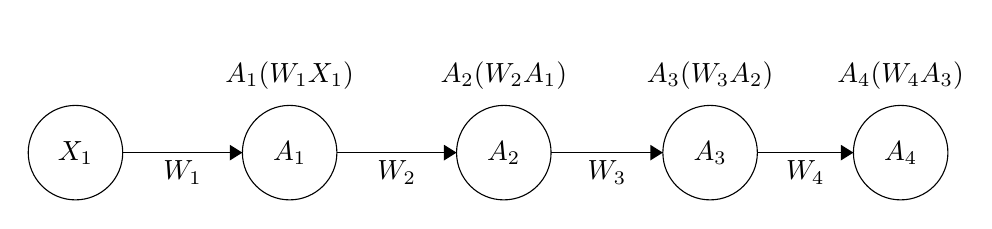
\begin{tikzpicture}[scale=0.2]
        \tikzstyle{every node}+=[inner sep=0pt]
        \draw [black] (16.1,-24.6) circle (3);
        \draw (16.1,-24.6) node {$X_1$};
        \draw [black] (29.7,-24.6) circle (3);
        \draw (29.7,-24.6) node {$A_1$};
        \draw [black] (43.3,-24.6) circle (3);
        \draw (43.3,-24.6) node {$A_2$};
        \draw [transparent] (29.7,-19.7) circle (3);
        \draw (29.7,-19.7) node {$A_1(W_1X_1)$};
        \draw [black] (56.4,-24.6) circle (3);
        \draw (56.4,-24.6) node {$A_3$};
        \draw [transparent] (43.3,-19.7) circle (3);
        \draw (43.3,-19.7) node {$A_2(W_2A_1)$};
        \draw [transparent] (56.4,-19.7) circle (3);
        \draw (56.4,-19.7) node {$A_3(W_3A_2)$};
        \draw [black] (68.5,-24.6) circle (3);
        \draw (68.5,-24.6) node {$A_4$};
        \draw [transparent] (68.5,-19.7) circle (3);
        \draw (68.5,-19.7) node {$A_4(W_4A_3)$};
        \draw [black] (19.1,-24.6) -- (26.7,-24.6);
        \fill [black] (26.7,-24.6) -- (25.9,-24.1) -- (25.9,-25.1);
        \draw (22.9,-25.1) node [below] {$W_1$};
        \draw [black] (32.7,-24.6) -- (40.3,-24.6);
        \fill [black] (40.3,-24.6) -- (39.5,-24.1) -- (39.5,-25.1);
        \draw (36.5,-25.1) node [below] {$W_2$};
        \draw [black] (46.3,-24.6) -- (53.4,-24.6);
        \fill [black] (53.4,-24.6) -- (52.6,-24.1) -- (52.6,-25.1);
        \draw (49.85,-25.1) node [below] {$W_3$};
        \draw [black] (59.4,-24.6) -- (65.5,-24.6);
        \fill [black] (65.5,-24.6) -- (64.7,-24.1) -- (64.7,-25.1);
        \draw (62.45,-25.1) node [below] {$W_4$};
        \end{tikzpicture}
    \end{center}
    \caption{A 4 layer network with a single-weight each layer}
    \label{fig:backprop_network}
\end{figure}

Now recall the equation for the gradient descent update step as well as the gradient of loss from the previous lectures:

\begin{align}
    W = W - \alpha \frac{\partial \Loss}{\partial W}
\end{align}

\begin{align}
    \nabla_W \text{Loss} = \frac{\partial \Loss}{\partial W} = \left( \frac{\partial \Loss}{\partial w_1},\, \frac{\partial \Loss}{\partial w_2},\, \ldots,\, \frac{\partial \Loss}{\partial w_m} \right)
\end{align}

Previously, we solved this using the chain rule:
\begin{align}
    \frac{\partial L}{\partial w_j} = \frac{\partial \hat{y}}{\partial w_j} \frac{\partial L}{\partial \hat{y}}
\end{align}

We can extend this chain rule technique and apply it to our network in \autoref{fig:backprop_network}. The idea is to consider all the terms that depend on each other in the network. The reason why we need to do this is because the input of a layer is the output of the previous layer. For example, changing $w_2$ will affect $A_4$, $A_3$, $A_2$, $A_1$, and $L$ so we must consider all these variables when we try to find $\frac{\partial L}{\partial w_1}$. We can do this by multiplying all the partial derivatives along the path from loss to $w_1$:

\begin{align}
    \frac{\partial L}{\partial w_4} = \color{blue} \frac{\partial L}{\partial A_4} \color{black} \cdot \frac{\partial A_4}{\partial w_4}
\end{align}
\begin{align}
    \frac{\partial L}{\partial w_3} = \color{blue} \frac{\partial L}{\partial A_4} \cdot \frac{\partial A_4}{\partial A_3} \color{black} \cdot \frac{\partial A_3}{\partial w_3}
\end{align}
\begin{align}
    \frac{\partial L}{\partial w_2} = \color{blue} \frac{\partial L}{\partial A_4} \cdot \frac{\partial A_4}{\partial A_3} \cdot \frac{\partial A_3}{\partial A_2} \color{black} \cdot \frac{\partial A_2}{\partial w_2}
\end{align}
\begin{align}
    \frac{\partial L}{\partial w_1} = \color{blue} \frac{\partial L}{\partial A_4} \cdot \frac{\partial A_4}{\partial A_3} \cdot \frac{\partial A_3}{\partial A_2} \cdot \frac{\partial A_2}{\partial A_1} \color{black} \cdot \frac{\partial A_1}{\partial w_1}
\end{align}

Observe that a lot of the partial derivattives are repeated, as colored in blue, this will be important in a bit. From the above, we can see that the partial derivatives generally comes in three forms. Each can be solved likeso (note that $A_{m-1}$ of the first layer is just the input $X$):

\begin{proof}
    Solve $\frac{\partial L}{\partial A_m}$ for MSE loss function. Recall that MSE for SGD $= \frac{1}{2}(y - \hat{y})^2$,
    \begin{align*}
      \frac{\partial L}{\partial A_m} &= 2 \cdot \frac{1}{2} \cdot (y - A_m) \cdot (-1)  &&\text{(chain rule)} \\
      &= A_m - y &&\qedhere\\
    \end{align*}
\end{proof}

\begin{proof}
    Solve $\frac{\partial A_{m+1}}{\partial A_{m}}$ for the sigmoid activation function. Recall that the derivative of the sigmoid function is $\sigma(x) \cdot [1-\sigma(x)]$ and that $A_{m+1} = \sigma (w_{m+1} \cdot A_{m})$.
    \begin{align*}
        \frac{\partial A_{m+1}}{\partial A_{m}} &= \sigma(A_{m}) \cdot [1 - \sigma(A_{m})] \cdot w_{m+1} &&\text{(derivative of sigmoid function)} \qedhere\\
    \end{align*}
\end{proof}

\begin{proof}
    Solve $\frac{\partial A_m}{\partial w_m}$. Recall that $A_m = \sigma (w_m \cdot A_{m-1})$:
    \begin{align*}
        \frac{\partial A_m}{\partial w_m} &= \sigma(A_{m-1}) \cdot [1 - \sigma(A_{m-1})] \cdot A_{m-1} \qedhere
    \end{align*}
\end{proof}

First, notice how the calculation of the partial derivatives of each layer can be computed locally. For example, the partial derivative of $\frac{\partial A_{m+1}}{\partial A_{m}}$ can be computed in the $(m+1)^{\text{th}}$ layer since the input $A_{m}$ and weight $w_{m+1}$ is known after the forward pass. Similarly, the partial derivative of $\frac{\partial A_m}{\partial w_m}$ can be calculated in the $m^{\text{th}}$ layer since the input to the $m^{\text{th}}$ layer is known. Finally, the partial derivatives in $\frac{\partial L}{\partial W} = \{ \frac{\partial L}{\partial w_1}, \cdots , \frac{\partial L}{\partial w_m}\}$ has a lot of repeated calculations (as colored in blue). Instead of recomputing the chain at each layer, we can keep track of this chain and continue multiplying onto it. This is also why we want to start at the last layer of the network (e.g $\frac{\partial L}{\partial w_m}$) and go backwards until the first layer (e.g $\frac{\partial L}{\partial w_1}$), hence the name \emph{backpropagation}.


%  This calculation doesn't depend on the other gates in the network, and it doesn't require knowledge of the overall structure of the network. Instead, each gate can compute its local gradient independently and pass it along to the gates that feed into it. This makes backpropagation a highly parallelizable and efficient process.

% Notice that backpropagation is a beautifully local process. Every gate in a circuit diagram gets some inputs and can right away compute two things: 1. its output value and 2. the local gradient of its inputs with respect to its output value. Notice that the gates can do this completely independently without being aware of any of the details of the full circuit that they are embedded in


% Vanishing and Exploding gradients


\begin{thebibliography}{2}
    \bibitem{DrCoop} Cooper.

    \bibitem{Stanford} Fei-Fei Li, Jiajun Wu, and Ruohan Gao, Stanford CS231n, Spring 2022. \url{https://web.archive.org/web/20230109135558/https://cs231n.github.io/}

    \bibitem{ActivationGraphs} Graphs of tanh, sigmoid, ReLU. \url{https://studymachinelearning.com/activation-functions-in-neural-network/}

\end{thebibliography}

\end{document}
